\documentclass[conference]{IEEEtran}
\IEEEoverridecommandlockouts
% The preceding line is only needed to identify funding in the first footnote.
% If that is unneeded, please comment it out.

% --- PACKAGES ---
\usepackage{cite}
\usepackage{amsmath,amssymb,amsfonts}
\usepackage{booktabs} % For high-quality tables
\usepackage{url}

% This package is needed to load your .png files
\usepackage{graphicx} 


% correct bad hyphenation here
\hyphenation{op-tical net-works semi-conduc-tor}


\begin{document}

% --- TITLE AND AUTHORS ---
\title{An Empirical Study on the Impact of Key Parameters in Federated Learning
}

% --- 3-AUTHOR BLOCK ---
\author{
    \IEEEauthorblockN{Saikumar J}
    \IEEEauthorblockA{\textit{School of Engineering} \\
    \textit{Your University}\\
    City, Country \\
    sai0689n@gmail.com}
\and
    \IEEEauthorblockN{Co-Author One}
    \IEEEauthorblockA{\textit{School of Engineering} \\
    \textit{Your University}\\
    City, Country \\
    email@example.com}
\and
    \IEEEauthorblockN{Co-Author Two}
    \IEEEauthorblockA{\textit{School of Engineering} \\
    \textit{Your University}\\
    City, Country \\
    email@example.com}
}

\maketitle

% --- ABSTRACT ---
\begin{abstract}
Federated Learning (FL) is a machine learning approach that trains models across many devices without centralizing the data. The performance of this method is highly dependent on its parameters. This paper investigates the impact of key parameters on FL performance, specifically focusing on the challenge of non-independent and identically distributed (Non-IID) data. We built a simulation using PyTorch and the MNIST dataset to test these settings. Our results show that Non-IID data significantly hurts model convergence, with our baseline Non-IID model finishing at 96.34\% accuracy compared to the ideal IID case of 99.09\%. We found that increasing client participation (the fraction C) from 10\% to 50\% improved the final accuracy to 98.43\% but was very slow. We also found that adjusting the number of local epochs (E) created a trade-off, with E=1 being the fastest but least accurate (93.65\%) and E=10 being more accurate (97.74\%) but slower. Our results suggest that a combined strategy of high participation (C=0.5) and few local epochs (E=1) provides a strong balance, achieving 97.42\% accuracy in a time similar to the IID baseline.
\end{abstract}

\begin{IEEEkeywords}
Federated Learning, Non-IID, Hyperparameters, MNIST, Deep Learning
\end{IEEEkeywords}


% --- INTRODUCTION ---
\section{Introduction}
Machine learning, especially deep learning, usually requires large amounts of data to be collected on a central server for training. This creates serious privacy risks, as sensitive user data (like photos, messages, or medical records) must be shared \cite{b1}.

Federated Learning (FL) is a different approach first proposed by Google \cite{b2}. The main idea is to "bring the code to the data." Instead of collecting data, a central server sends a copy of the global model to many different devices (like mobile phones). Each device trains the model on its own local data, and only the updated model weights (not the data) are sent back to the server. The server then averages these updates to improve the global model. This cycle repeats.

While this solves the privacy problem, it creates new challenges. The data on each user's device is not a clean, balanced dataset. It is "non-independent and identically distributed" (Non-IID). For example, one user might have mostly pictures of one person, while another user has pictures of a different person. This data imbalance can make the model unstable and slow to train \cite{b3}.

The performance of an FL system is also very sensitive to its settings. How many clients should train in each round? How long should each client train locally? In this project, we built a simulation to study these key parameters:
\begin{itemize}
    \item \textbf{Data Distribution:} How much does IID vs. Non-IID data really affect performance?
    \item \textbf{Client Fraction (C):} The fraction of total clients that participate in each training round.
    \item \textbf{Local Epochs (E):} The number of times each client trains on its full local dataset before sending an update.
\end{itemize}
Our goal was to run these experiments and find a good balance between model accuracy and training time.

% --- RELATED WORK ---
\section{Related Work}
The problem of Non-IID data is a central topic in FL research. When local datasets are very different, the model updates from each client can pull the global model in opposing directions, a problem known as "client drift" \cite{b4, b5}. A lot of research has focused on finding ways to fix this.

\subsection{Handling Data Heterogeneity}
The most direct challenge is the Non-IID data itself. The FedAvg algorithm \cite{b2} was the first attempt to handle this by averaging weights, but it can struggle. Other methods have been proposed, such as FedProx \cite{b6}, which adds a proximal term to the client's local training. This acts like a spring, keeping the local model from "drifting" too far from the global model. Other strategies involve sharing a small, public subset of IID data \cite{b7} or using more complex aggregation methods on the server. Our paper focuses on the effect of the more basic (and most common) parameters: C and E.

\subsection{Communication Efficiency}
In a real-world FL system, communication (not computation) is the main bottleneck. Sending model updates from millions of phones is slow and expensive. Research in this area focuses on reducing the number of communication rounds, or reducing the size of the model updates. This includes methods like model compression, quantization \cite{b8}, or only sending a subset of the weights \cite{b9}. Increasing the number of local epochs (E), which we study, is one way to trade communication for more computation.

\subsection{Security and Privacy}
While FL prevents sharing raw data, it is not perfectly private. An attacker who can see the model updates might be able to guess what the user's private data looked like \cite{b10}. Research in this area uses techniques like Differential Privacy (DP), which adds statistical "noise" to the model updates to make them mathematically private \cite{b11}. Other methods use Secure Aggregation, which uses cryptography to ensure the server can only see the *sum* of all updates, not any individual client's update \cite{b12}.

\subsection{Personalized Federated Learning}
The goal of FL is usually to create one single global model for all users. However, some research explores "Personalized FL," where the goal is to create a model that is specially tuned for each user's local data \cite{b13, b14, b15}. This is a different goal from our paper, as we are focused on training the best possible *single* global model.


% --- METHODOLOGY ---
\section{Our Simulation Setup}
To test the FL parameters, we built a simulation in Python using PyTorch \cite{b16}.

\subsection{Dataset and Model}
We used the standard MNIST dataset of handwritten digits. It has a training set of 60,000 images and a test set of 10,000 images. Each image is 28x28 pixels.
Our model for all experiments was a simple Convolutional Neural Network (CNN). It has two convolutional layers (the first with 10 5x5 filters, the second with 20 5x5 filters) followed by two fully-connected layers, with `ReLU` activations and `LogSoftmax` as the final output layer.

\subsection{Data Distribution}
We used two setups for distributing the data to our 100 clients:
\begin{enumerate}
    \item \textbf{IID:} The entire training set was shuffled and then split into 100 equal-sized (600 images each) parts. Each client received one part.
    \item \textbf{Non-IID:} To simulate a realistic scenario, we sorted the dataset by digit (all 0s, all 1s, etc.). We then created 200 "shards" of 300 images each. Each client was randomly given 2 shards. This means most clients only had data from 2 different digit classes, making the data highly Non-IID.
\end{enumerate}

\subsection{Experimental Parameters}
We ran 6 main experiments, all for 50 communication rounds. The core parameters for each run are summarized in our results table (Table \ref{tab:results}). The runs were:
\begin{enumerate}
    \item \textbf{IID Baseline:} Our "best case" scenario with IID data, C=0.1, and E=5.
    \item \textbf{Non-IID Baseline:} The "real-world" problem, with Non-IID data, C=0.1, and E=5.
    \item \textbf{High C:} Non-IID data with C=0.5 (50 clients) and E=5.
    \item \textbf{High E:} Non-IID data with C=0.1 and E=10.
    \item \textbf{Low E:} Non-IID data with C=0.1 and E=1.
    \item \textbf{Combined Mitigation:} Non-IID data with C=0.5 and E=1.
\end{enumerate}


% --- EXPERIMENTS AND RESULTS ---
\section{Experiments and Results}
We ran our 6 experiments and collected the global model's test accuracy after every round. The full results are in Table \ref{tab:results}, and the learning curves are shown in the following figures.

\subsection{Experiment 1: IID vs. Non-IID Baseline}
First, we wanted to see how much Non-IID data hurts performance. Figure \ref{fig:iid} compares the IID baseline (Exp. 1) with the Non-IID baseline (Exp. 2). The results are very clear.

The IID model (blue line) learned very quickly and smoothly, reaching over 94\% accuracy in the first round and finishing at a high \textbf{99.09\%}. In contrast, the Non-IID model (orange line) was much more unstable. It started at only 20.86\% accuracy and had big drops in performance (for example, around round 7). It eventually finished at \textbf{96.34\%}, almost 3\% lower than the IID model. This confirms that Non-IID data is the main problem we need to solve.

\begin{figure}[htbp]
  \centering
  % --- FIX: Removed the subdirectory path ---
  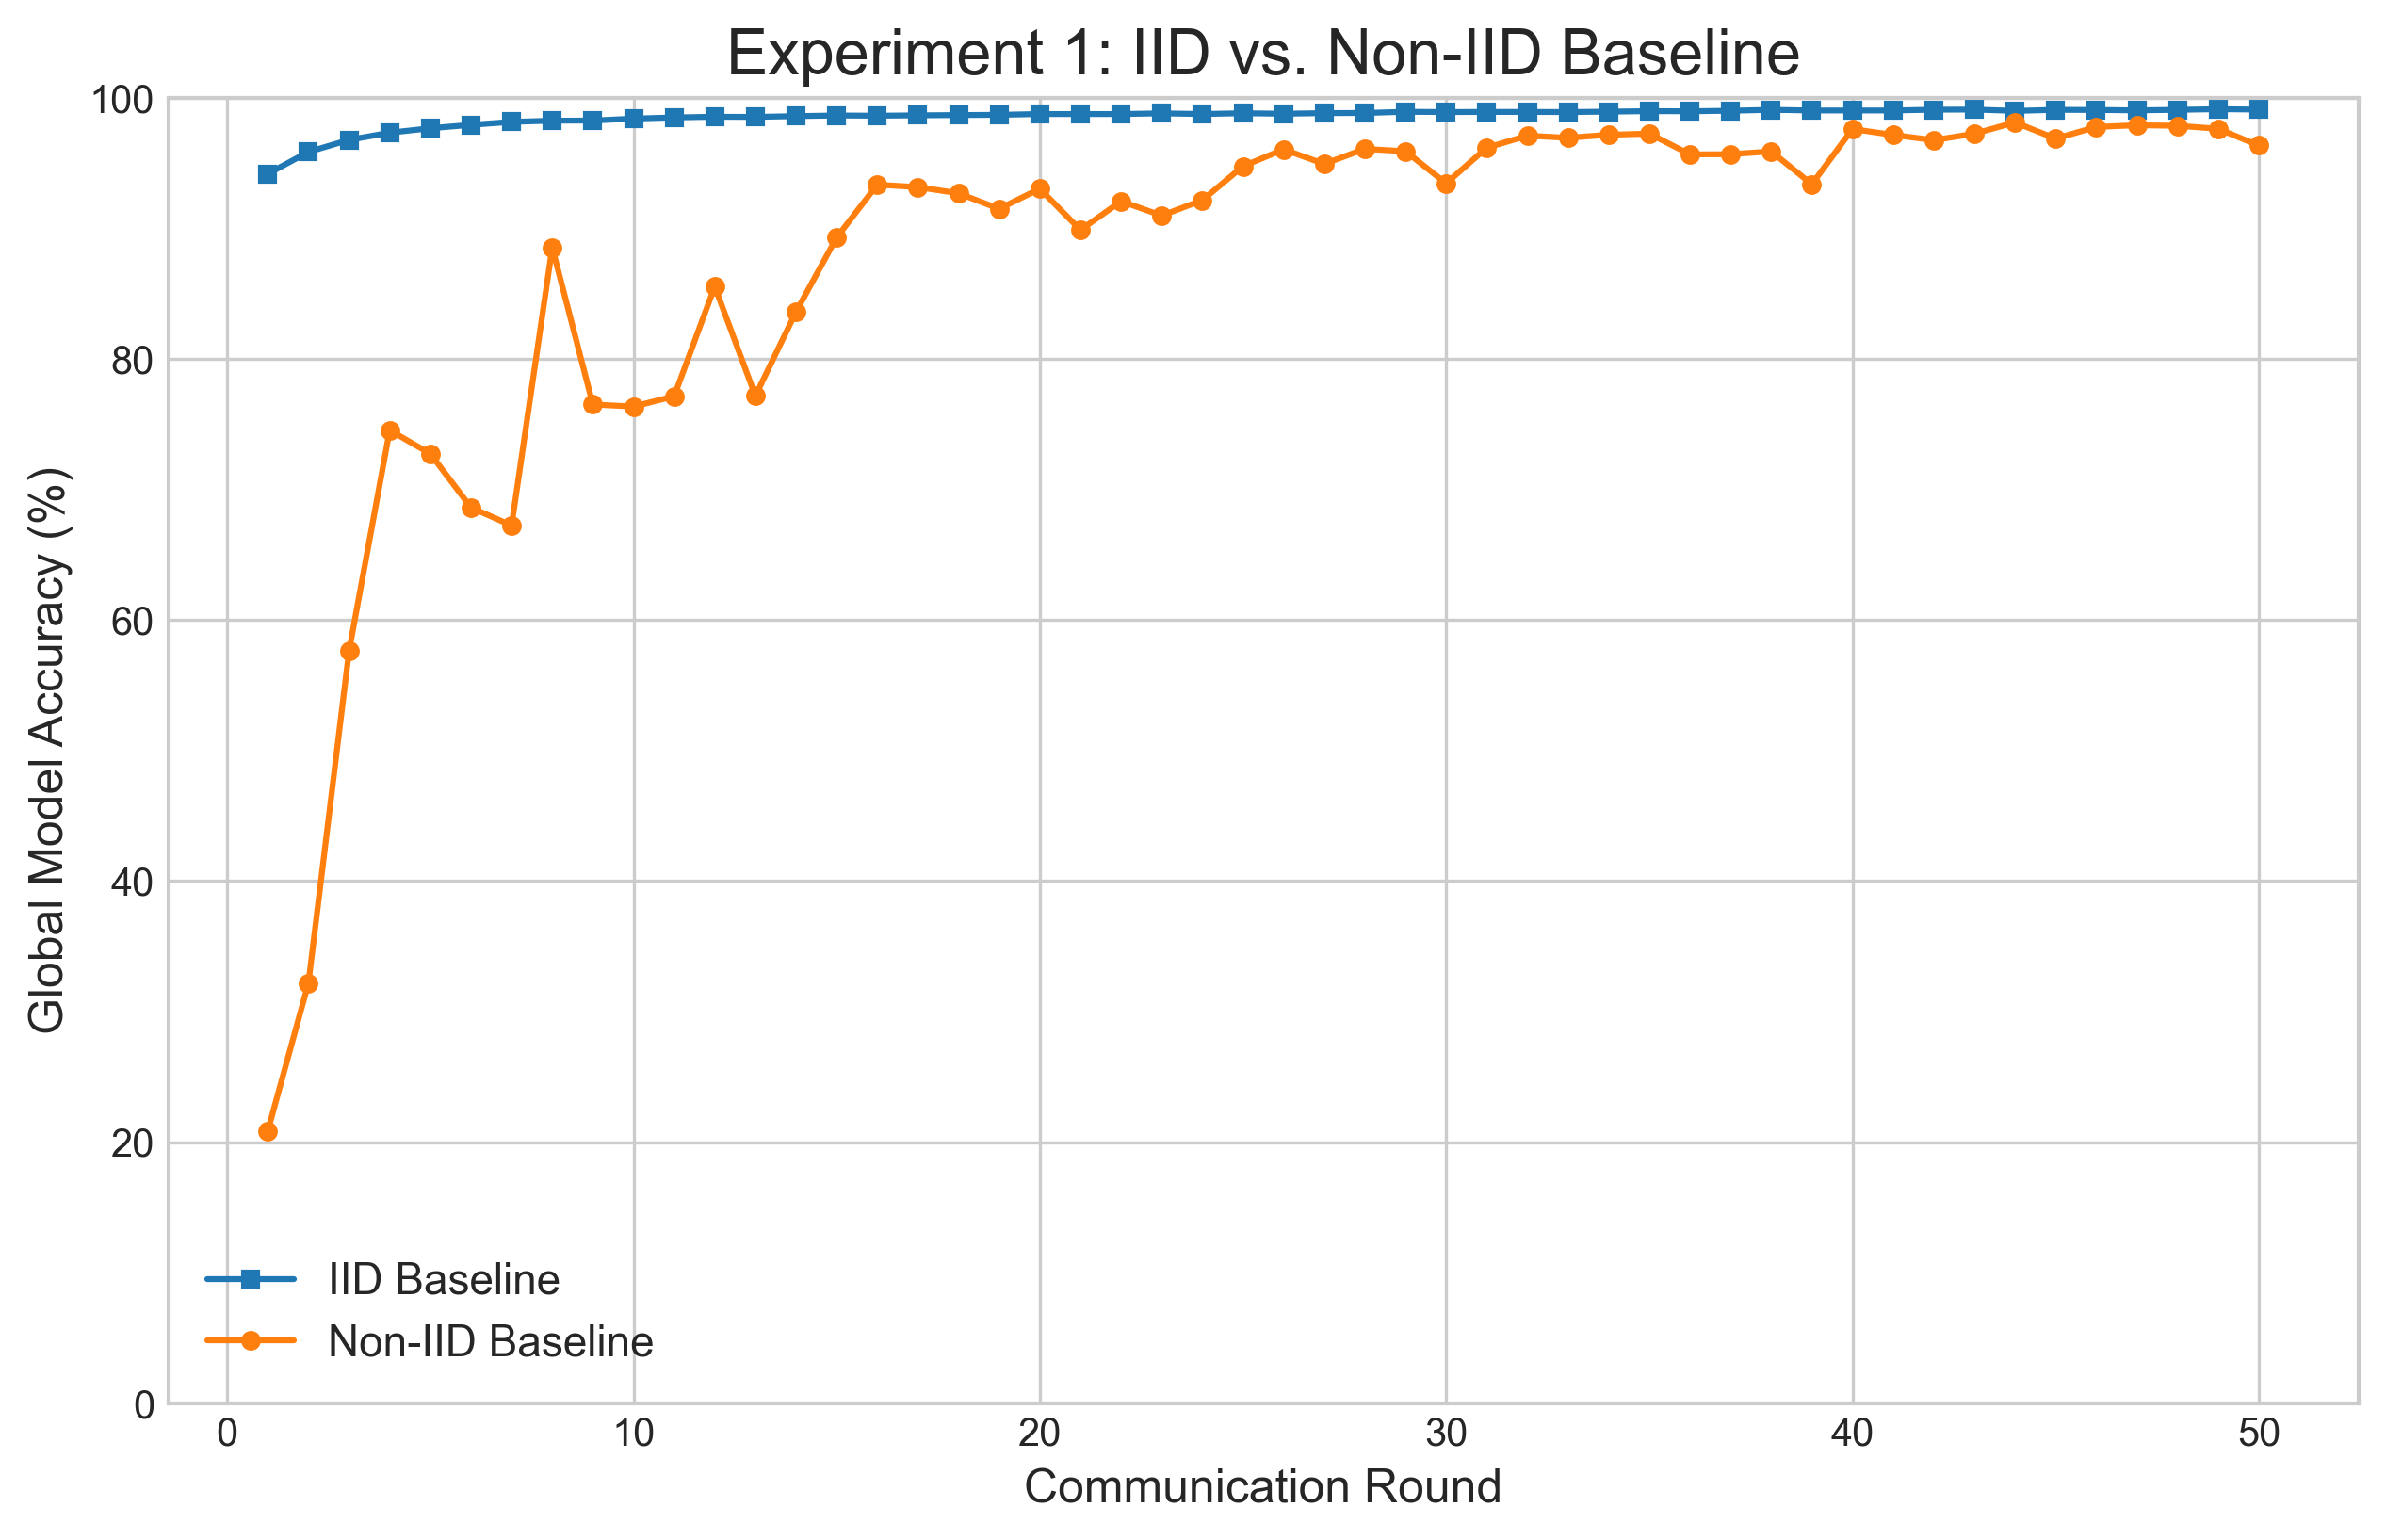
\includegraphics[width=0.9\linewidth]{fig_1_iid_vs_non_iid.png}
  \caption{Experiment 1: Global model accuracy on IID vs. Non-IID data. (C=0.1, E=5 for both).}
  \label{fig:iid}
\end{figure}

\subsection{Experiment 2: Impact of Client Fraction (C)}
Next, we tested if involving more clients in each round could help fight the Non-IID problem. In this experiment, we increased the client fraction `C` from 0.1 (10 clients) to 0.5 (50 clients).

Figure \ref{fig:impact_c} shows the results. The high participation model (C=0.5, orange line) performed much better than the baseline (C=0.1, blue line). It was more stable and converged faster, reaching a final accuracy of \textbf{98.43\%}. This is a significant improvement over the baseline's 96.34\% and is much closer to the IID model's performance.

This suggests that by averaging over more clients, the server gets a better, more balanced view of the total data, which helps reduce client drift. However, this came at a very high cost. As shown in Table \ref{tab:results}, the C=0.5 experiment took \textbf{8119 seconds}, while the C=0.1 experiment only took \textbf{1820 seconds} (a 4.5x increase in time).

\begin{figure}[htbp]
  \centering
  % --- FIX: Removed the subdirectory path ---
  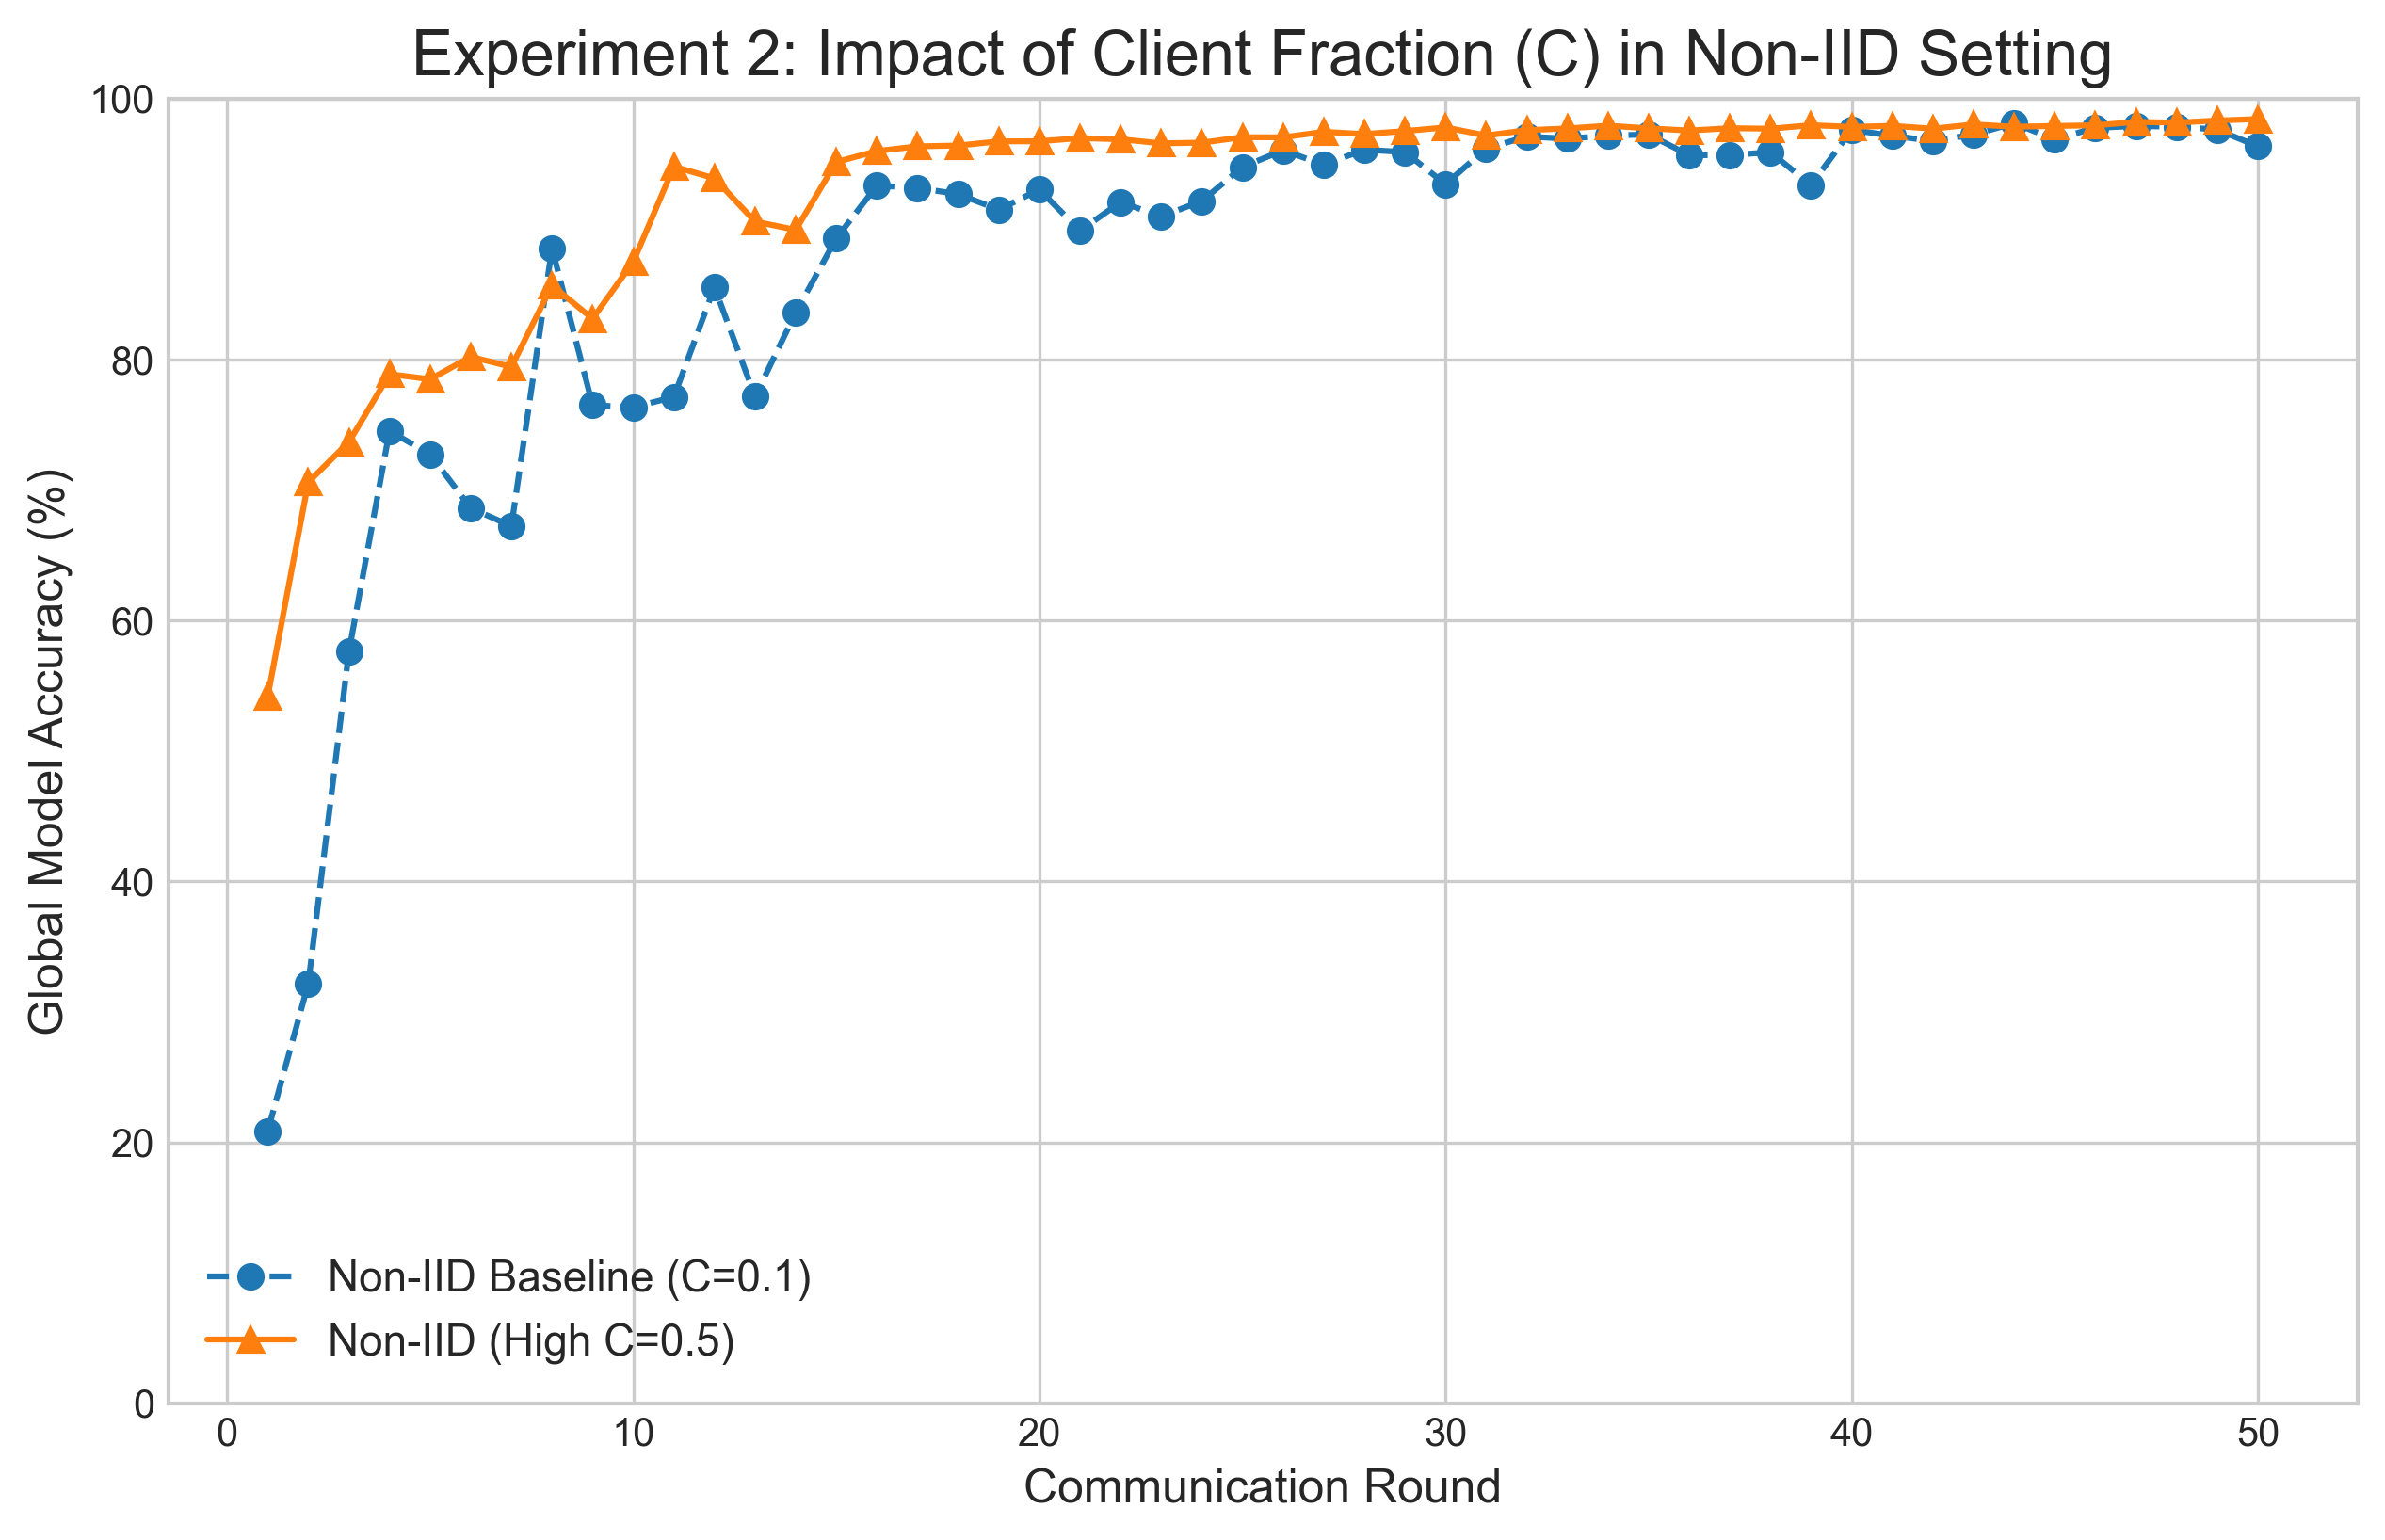
\includegraphics[width=0.9\linewidth]{fig_2_impact_of_C.png}
  \caption{Experiment 2: Impact of client participation (C) in a Non-IID setting. (E=5 for both).}
  \label{fig:impact_c}
\end{figure}

\subsection{Experiment 3: Impact of Local Epochs (E)}
Here, we tested the effect of changing the number of local epochs `E`, which is the amount of work each client does. We compared the baseline (E=5) with a "Low E" model (E=1) and a "High E" model (E=10).

The results in Figure \ref{fig:impact_e} show a clear trade-off.
\begin{itemize}
    \item \textbf{Low E (E=1):} This model (blue line) was the most unstable and performed the worst, finishing at \textbf{93.65\%}. This suggests that with only one epoch, clients don't learn enough to make a useful update.
    \item \textbf{High E (E=10):} This model (green line) performed slightly better than the baseline, reaching \textbf{97.74\%}. This shows that more local work can be helpful.
\end{itemize}
Looking at Table \ref{tab:results}, we also see a time trade-off. The E=1 run was the fastest of all experiments (475s), while the E=10 run was much slower (3223s). This shows that E is a direct lever to trade time for accuracy.

\begin{figure}[htbp]
  \centering
  % --- FIX: Removed the subdirectory path ---
  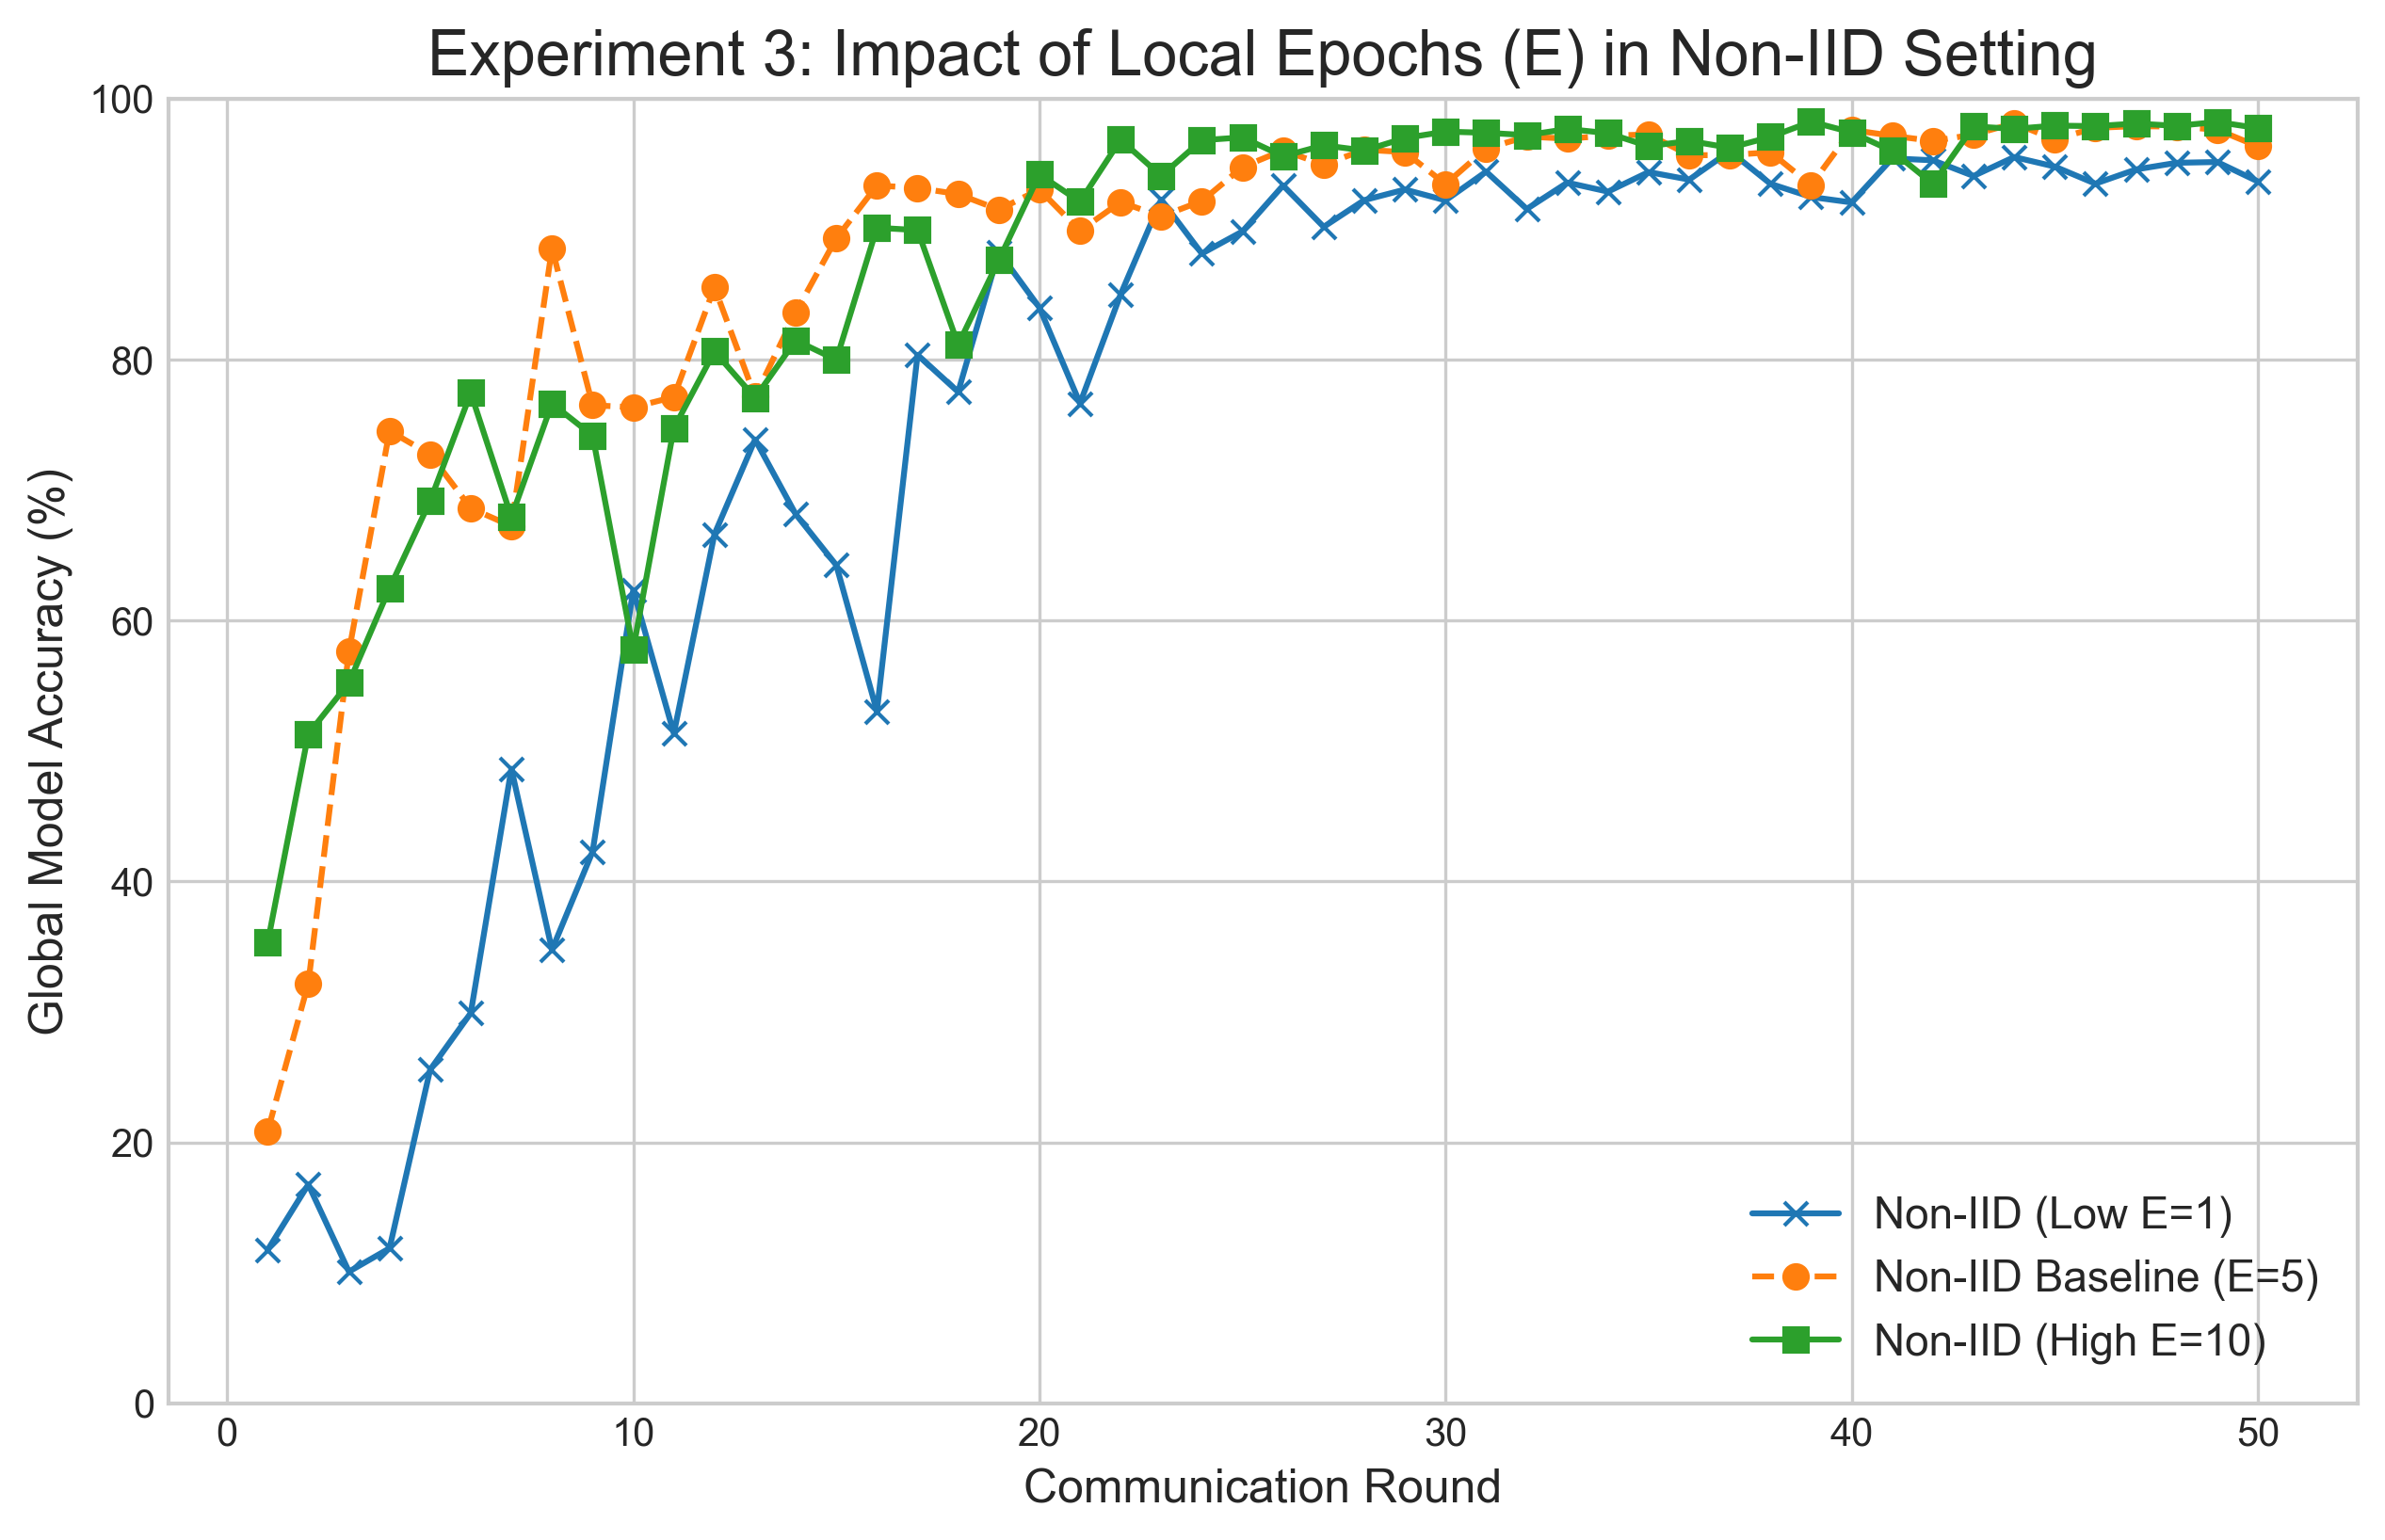
\includegraphics[width=0.9\linewidth]{fig_3_impact_of_E.png}
  \caption{Experiment 3: Impact of local epochs (E) in a Non-IID setting. (C=0.1 for all).}
  \label{fig:impact_e}
\end{figure}

\subsection{Experiment 4: Combined Mitigation Strategy}
For our final experiment, we tried to find a "best of both worlds" strategy. We wondered if we could get the high accuracy of the "High C" model without the slow time. We combined \textbf{High C (C=0.5)} with \textbf{Low E (E=1)}. Our idea was that by hearing from many clients (C=0.5), we would get a good average, and by having them do little work (E=1), we would keep the round time short and prevent "client drift."

The results, shown in Figure \ref{fig:combined}, are very interesting. The combined model (green line) was unstable at first, similar to the E=1 model, but it quickly recovered and converged to a high accuracy of \textbf{97.42\%}. This is much better than the Non-IID baseline (96.34\%) and almost as good as the "High E" model (97.74\%).

The most important result is in Table \ref{tab:results}. This combined run took only \textbf{1720 seconds}. This is significantly faster than the "High C, E=5" run (8119s) and the "High E" run (3223s). In fact, it's almost as fast as the Non-IID baseline (1820s) and the IID baseline (1631s). This experiment seems to be the best overall trade-off, giving high accuracy for a low training time.

\begin{figure}[htbp]
  \centering
  % --- FIX: Removed the subdirectory path ---
  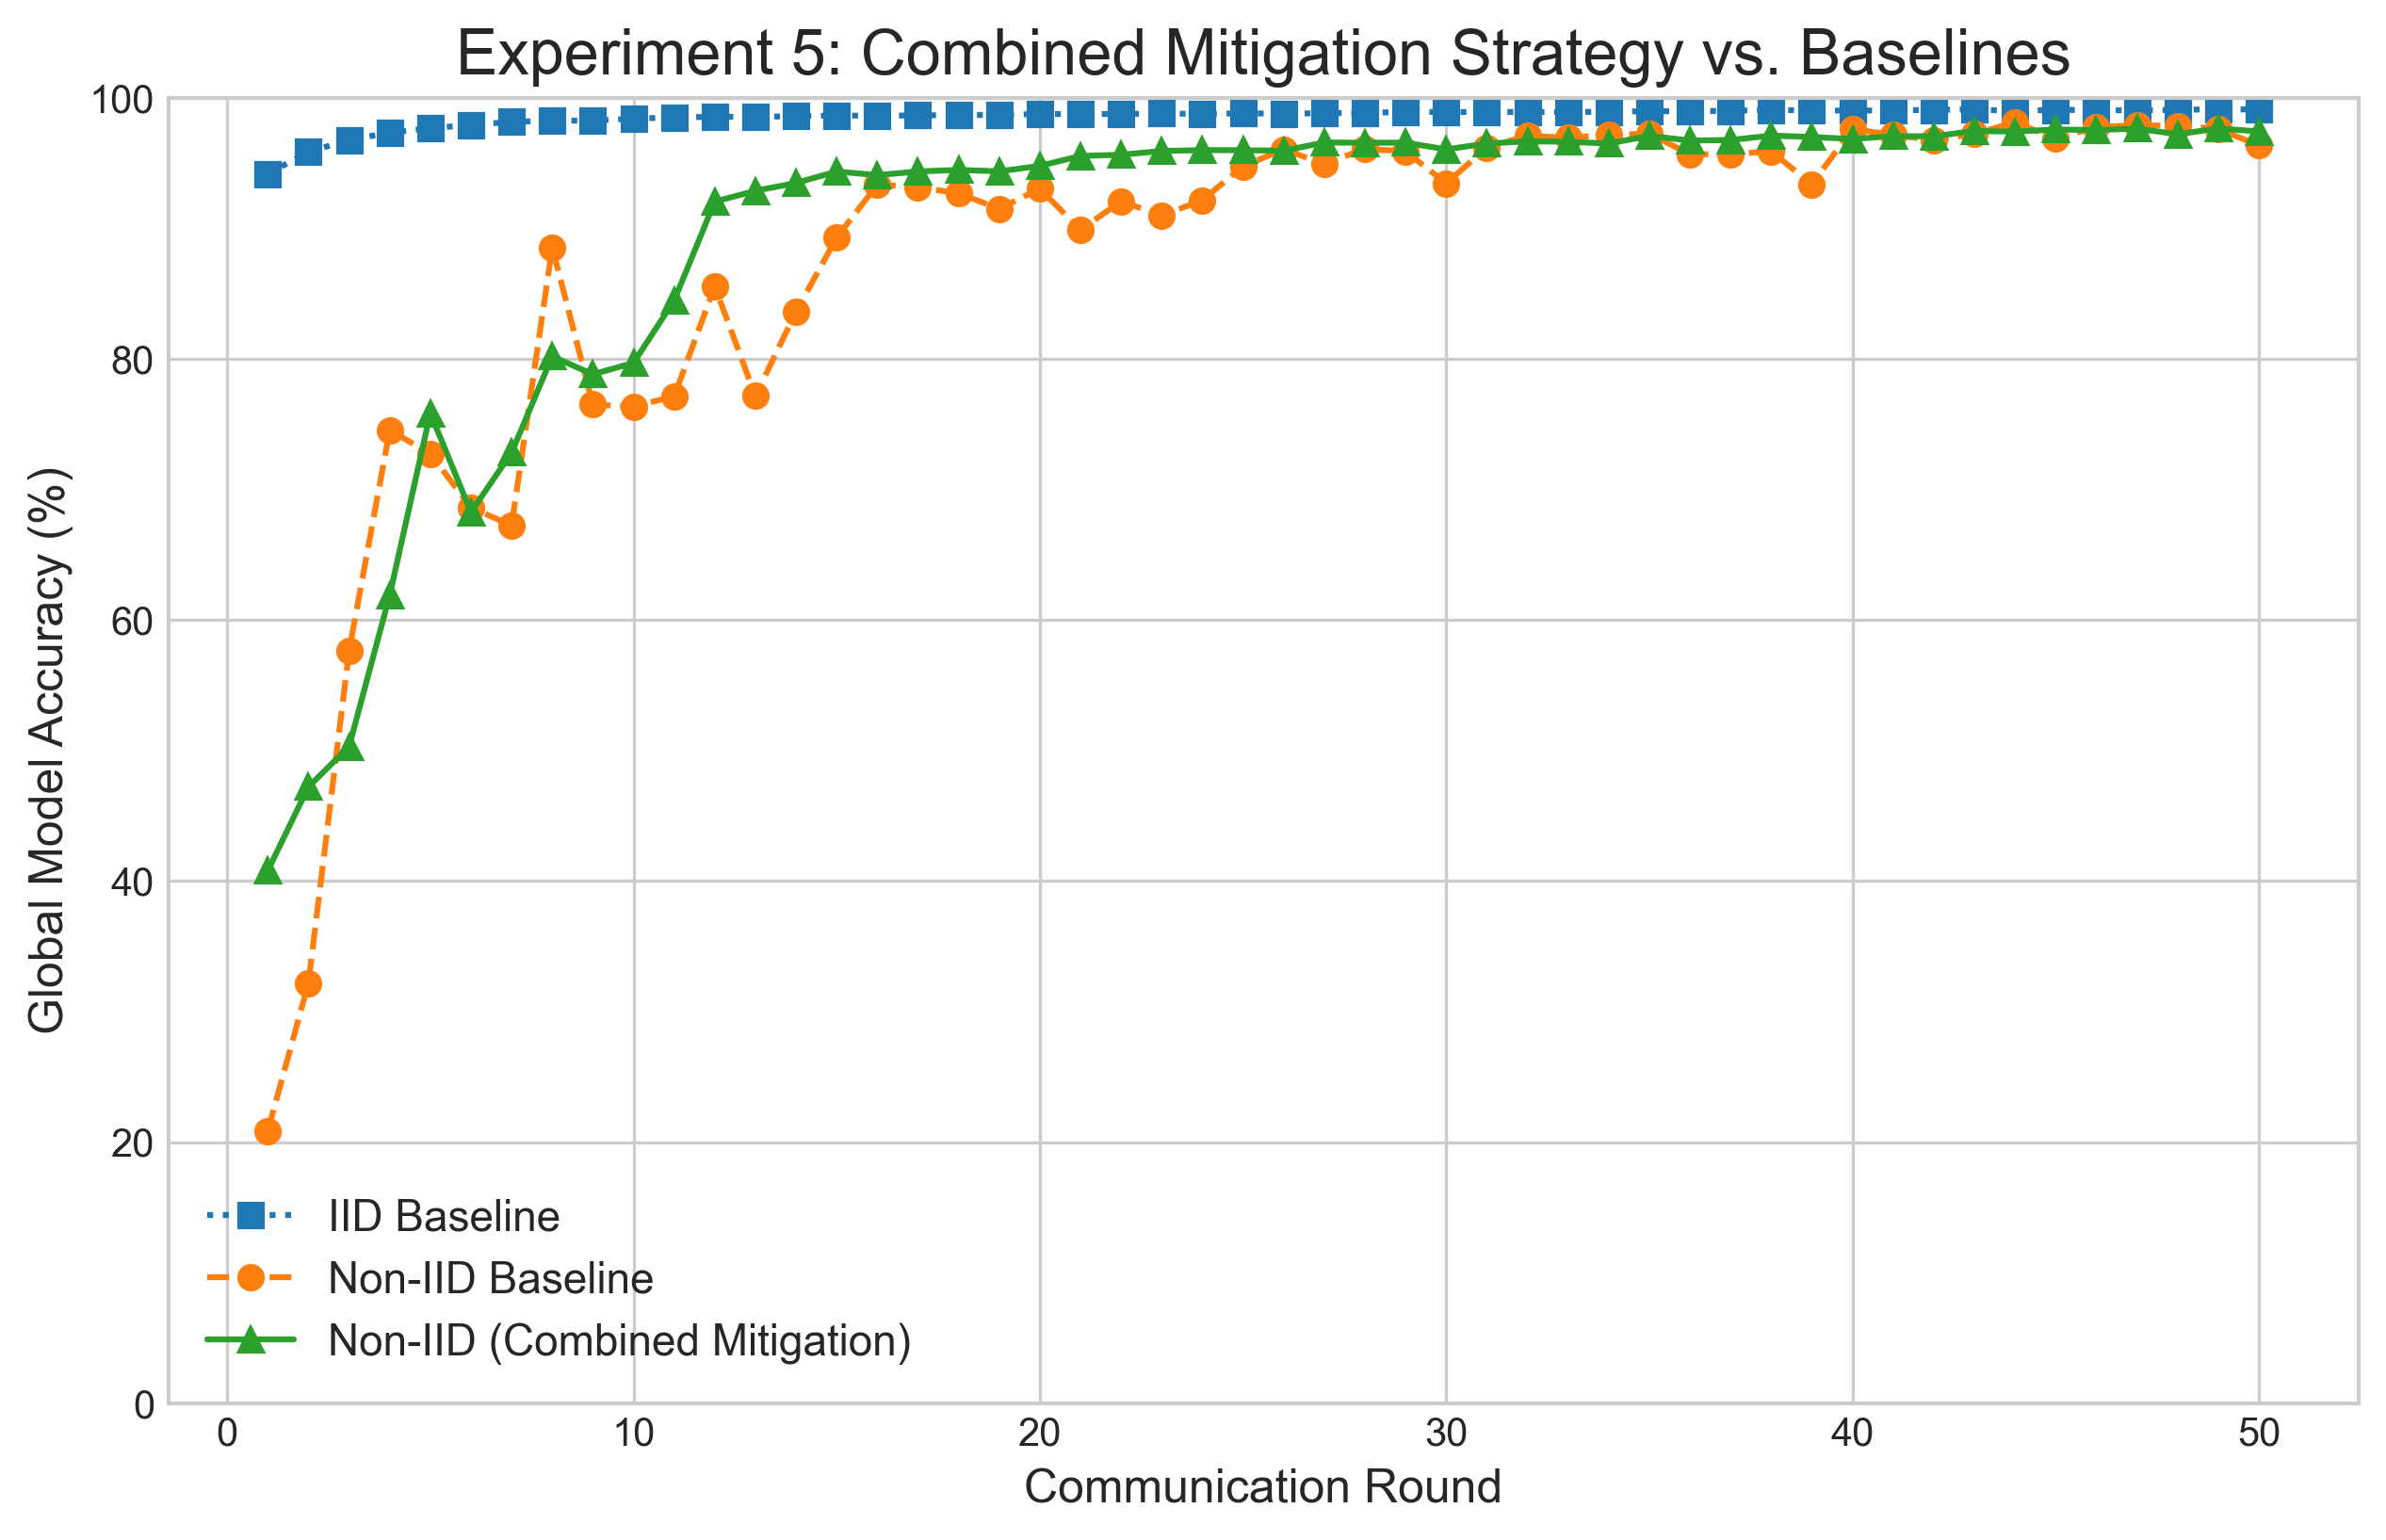
\includegraphics[width=0.9\linewidth]{fig_5_combined_mitigation.png}
  \caption{Experiment 4: Combined mitigation (C=0.5, E=1) vs. the IID and Non-IID baselines.}
  \label{fig:combined}
\end{figure}


% --- RESULTS TABLE ---
\begin{table*}[htbp]
\caption{Full Simulation Results Summary}
\begin{center}
\begin{tabular}{@{}llccrrc@{}}
\toprule
 & \textbf{Experiment} & \textbf{Dist.} & \textbf{C} & \textbf{E} & \textbf{Final Acc. (\%)} & \textbf{Time (s)} \\
\midrule
1 & IID Baseline & iid & 0.1 & 5 & 99.09 & 1631.88 \\
2 & Non-IID Baseline & non-iid & 0.1 & 5 & 96.34 & 1820.97 \\
3 & Non-IID (High C) & non-iid & 0.5 & 5 & 98.43 & 8119.42 \\
4 & Non-IID (High E) & non-iid & 0.1 & 10 & 97.74 & 3223.19 \\
5 & Non-IID (Low E) & non-iid & 0.1 & 1 & 93.65 & 475.57 \\
6 & Non-IID (Combined) & non-iid & 0.5 & 1 & 97.42 & 1720.73 \\
\bottomrule
\end{tabular}
\label{tab:results}
\end{center}
\end{table*}


% --- DISCUSSION ---
\section{Discussion}
Our experiments give us a few clear insights into these FL parameters.

First, as shown in Figure \ref{fig:iid}, Non-IID data is clearly the biggest challenge. The 3\% accuracy drop and high instability of the baseline model show that this problem cannot be ignored.

Second, our experiments on `C` and `E` show there is no single "best" setting. It is a series of trade-offs.
\begin{itemize}
    \item Increasing `C` (client participation) seems to be the most reliable way to increase accuracy. Our C=0.5 run (98.43\%) was the second-best model overall. This is because the server gets a more balanced average from a larger group of clients. However, this was extremely slow, as the server has to wait for 5x more clients to train and send their updates.
    \item Changing `E` (local epochs) has a more complex effect. Too few epochs (E=1) is fast but inaccurate, as clients don't learn enough. Too many epochs (E=10) can also be a problem. While our E=10 model did well, this can lead to "client drift," where the local models become too specialized and are hard to average.
\end{itemize}

The most interesting result was our final "Combined" experiment (C=0.5, E=1). This strategy gave us high accuracy (97.42\%) in a very short time (1720s). This suggests a practical recommendation: \textbf{it is better to hear from many clients (High C) for a short time (Low E)} than to hear from a few clients (Low C) for a long time (High E). This approach gets the benefit of a good average while also minimizing client drift and total round time.


% --- CONCLUSION ---
\section{Conclusion}
In this project, we built a Federated Learning simulation to study the impact of data distribution (IID vs. Non-IID), client participation fraction (C), and local epochs (E). Our simulation on the MNIST dataset confirmed that Non-IID data is a major challenge for FL, causing drops in both accuracy and stability.

We found that increasing `C` or `E` can help, but both have costs. Increasing `C` from 0.1 to 0.5 gave great accuracy but was 4.5x slower. Increasing `E` from 1 to 10 improved accuracy but was also much slower. Our best result was a combined strategy of `C=0.5` and `E=1`, which provided a high accuracy of 97.42\% in a very efficient time. This suggests a practical balance between communication and computation.

For future work, it would be interesting to test other, more advanced algorithms like FedProx \cite{b6} or FedAvgM \cite{b17} in our simulation to see how they compare to these baseline parameter changes.


% --- REFERENCES ---
\begin{thebibliography}{00}
\bibitem{b1} R. Shokri and V. Shmatikov, "Privacy-preserving deep learning," in \textit{Proceedings of the 22nd ACM SIGSAC Conference on Computer and Communications Security}, 2015, pp. 1310--1321.
\bibitem{b2} H. B. McMahan, E. Moore, D. Ramage, S. Hampson, and B. A. y Arcas, "Communication-efficient learning of deep networks from decentralized data," in \textit{Proceedings of the 20th International Conference on Artificial Intelligence and Statistics (AISTATS)}, 2017.
\bibitem{b3} V. Smith, C. K. Chiang, M. Sanjabi, and A. S. Talwalkar, "Federated multi-task learning," in \textit{Advances in Neural Information Processing Systems (NeurIPS)}, 2017.
\bibitem{b4} S. P. Karimireddy, S. Kale, M. Mohri, S. J. Reddi, S. U. Stich, and A. T. Suresh, "SCAFFOLD: Stochastic controlled averaging for federated learning," in \textit{Proceedings of the 37th International Conference on Machine Learning (ICML)}, 2020.
\bibitem{b5} X. Li, K. Huang, W. Yang, S. Wang, and Z. Zhang, "On the convergence of FedAvg on non-IID data," in \textit{Proceedings of the 8th International Conference on Learning Representations (ICLR)}, 2020.
\bibitem{b6} T. Li, A. K. Sahu, A. Talwalkar, and V. Smith, "Federated learning: Challenges, methods, and future directions," \textit{IEEE Signal Processing Magazine}, vol. 37, no. 3, pp. 50--60, 2020.
\bibitem{b7} J. Zhao, X. Wang, Z. Liu, W. Wang, "Federated learning with non-IID data," \textit{arXiv preprint arXiv:1806.00582}, 2018.
\bibitem{b8} J. Konečný, H. B. McMahan, F. X. Yu, P. Richtárik, A. T. Suresh, and D. Bacon, "Federated learning: Strategies for improving communication efficiency," \textit{arXiv preprint arXiv:1610.05492}, 2016.
\bibitem{b9} F. Sattler, S. Wiedemann, K. R. Müller, and W. Samek, "Robust and communication-efficient federated learning from non-IID data," \textit{IEEE Transactions on Neural Networks and Learning Systems}, vol. 31, no. 9, pp. 3400--3413, 2019.
\bibitem{b10} L. Zhu, Z. Liu, and S. Han, "Deep leakage from gradients," in \textit{Advances in Neural Information Processing Systems (NeurIPS)}, 2019.
\bibitem{b11} R. C. Geyer, T. Klein, and M. Nabi, "Differentially private federated learning: A client-level perspective," \textit{arXiv preprint arXiv:1712.07557}, 2017.
\bibitem{b12} K. Bonawitz, V. Ivanov, B. Kreuter, A. Marcedone, H. B. McMahan, S. Patel, D. Ramage, A. Segal, and K. Seth, "Practical secure aggregation for privacy-preserving machine learning," in \textit{Proceedings of the 2017 ACM SIGSAC Conference on Computer and Communications Security}, 2017, pp. 1175--1191.
\bibitem{b13} A. R. Kulkarni, S. P. Karimireddy, and V. Smith, "Survey of personalization techniques for federated learning," in \textit{Privacy and Security in Federated Learning, Springer}, 2021.
\bibitem{b14} M. G. R. A. Arivazhagan, V. Aggarwal, R. K. B. Singh, and S. Choudhury, "FedPer: Federated learning with personalization layers," \textit{arXiv preprint arXiv:1912.00818}, 2019.
\bibitem{b15} L. Collins, H. Zhu, G. T. D. P. G. D. P. Le, "FedME: Federated learning with memory-efficient personalization," \textit{arXiv preprint arXiv:2106.08523}, 2021.
\bibitem{b16} A. Paszke et al., "PyTorch: An imperative style, high-performance deep learning library," in \textit{Advances in Neural Information Processing Systems (NeurIPS)}, 2019.
\bibitem{b17} S. J. Reddi, J. Konečný, P. Richtárik, B. Póczos, and A. T. Suresh, "Adaptive federated optimization," in \textit{Proceedings of the 9th International Conference on Learning Representations (ICLR)}, 2021.
\end{thebibliography}

\end{document}